% !TEX root = ../../I4PRJ, Grp3 - Rapport.tex
\chapter{Arkitektur}
I dette afsnit beskrives den overordnede arkitektur for systemet. Systemets arkitektur har dannet ramme for design og senere implementering. Domæneanalyse giver anledning til en 3-tier arkitektur, da systemet har tre domæner, som er application, server og database.

\section{3 Tier Model}
\begin{figure}
	\centering
	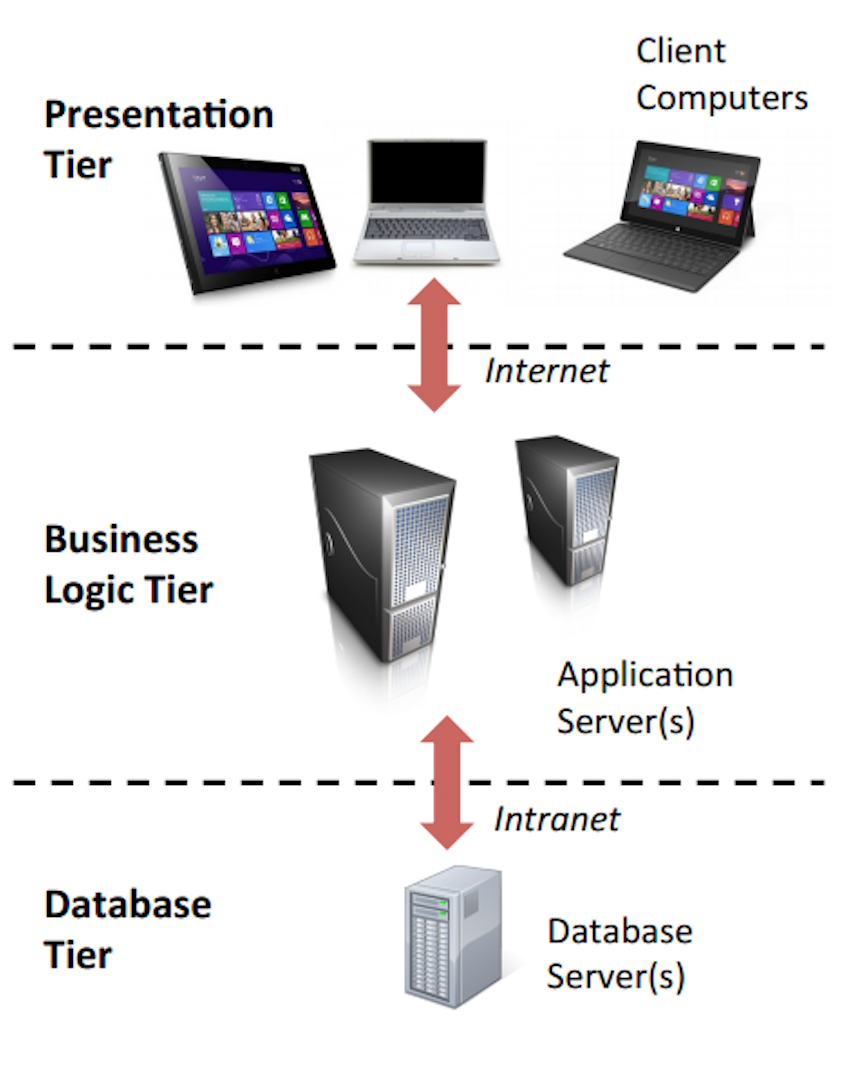
\includegraphics[width=0.5\linewidth]{figs/arkitektur/3tier}
	\caption{ 3-Tier}
	\label{fig:3tier}
\end{figure}

Figur~\ref{fig:3tier} viser tre tiers, som repræsenterer hvert sit ansvarsområde, som ønskes afkoblet. I det følgende vil de tre tiers blive beskrevet.

\begin{figure}
	\centering
	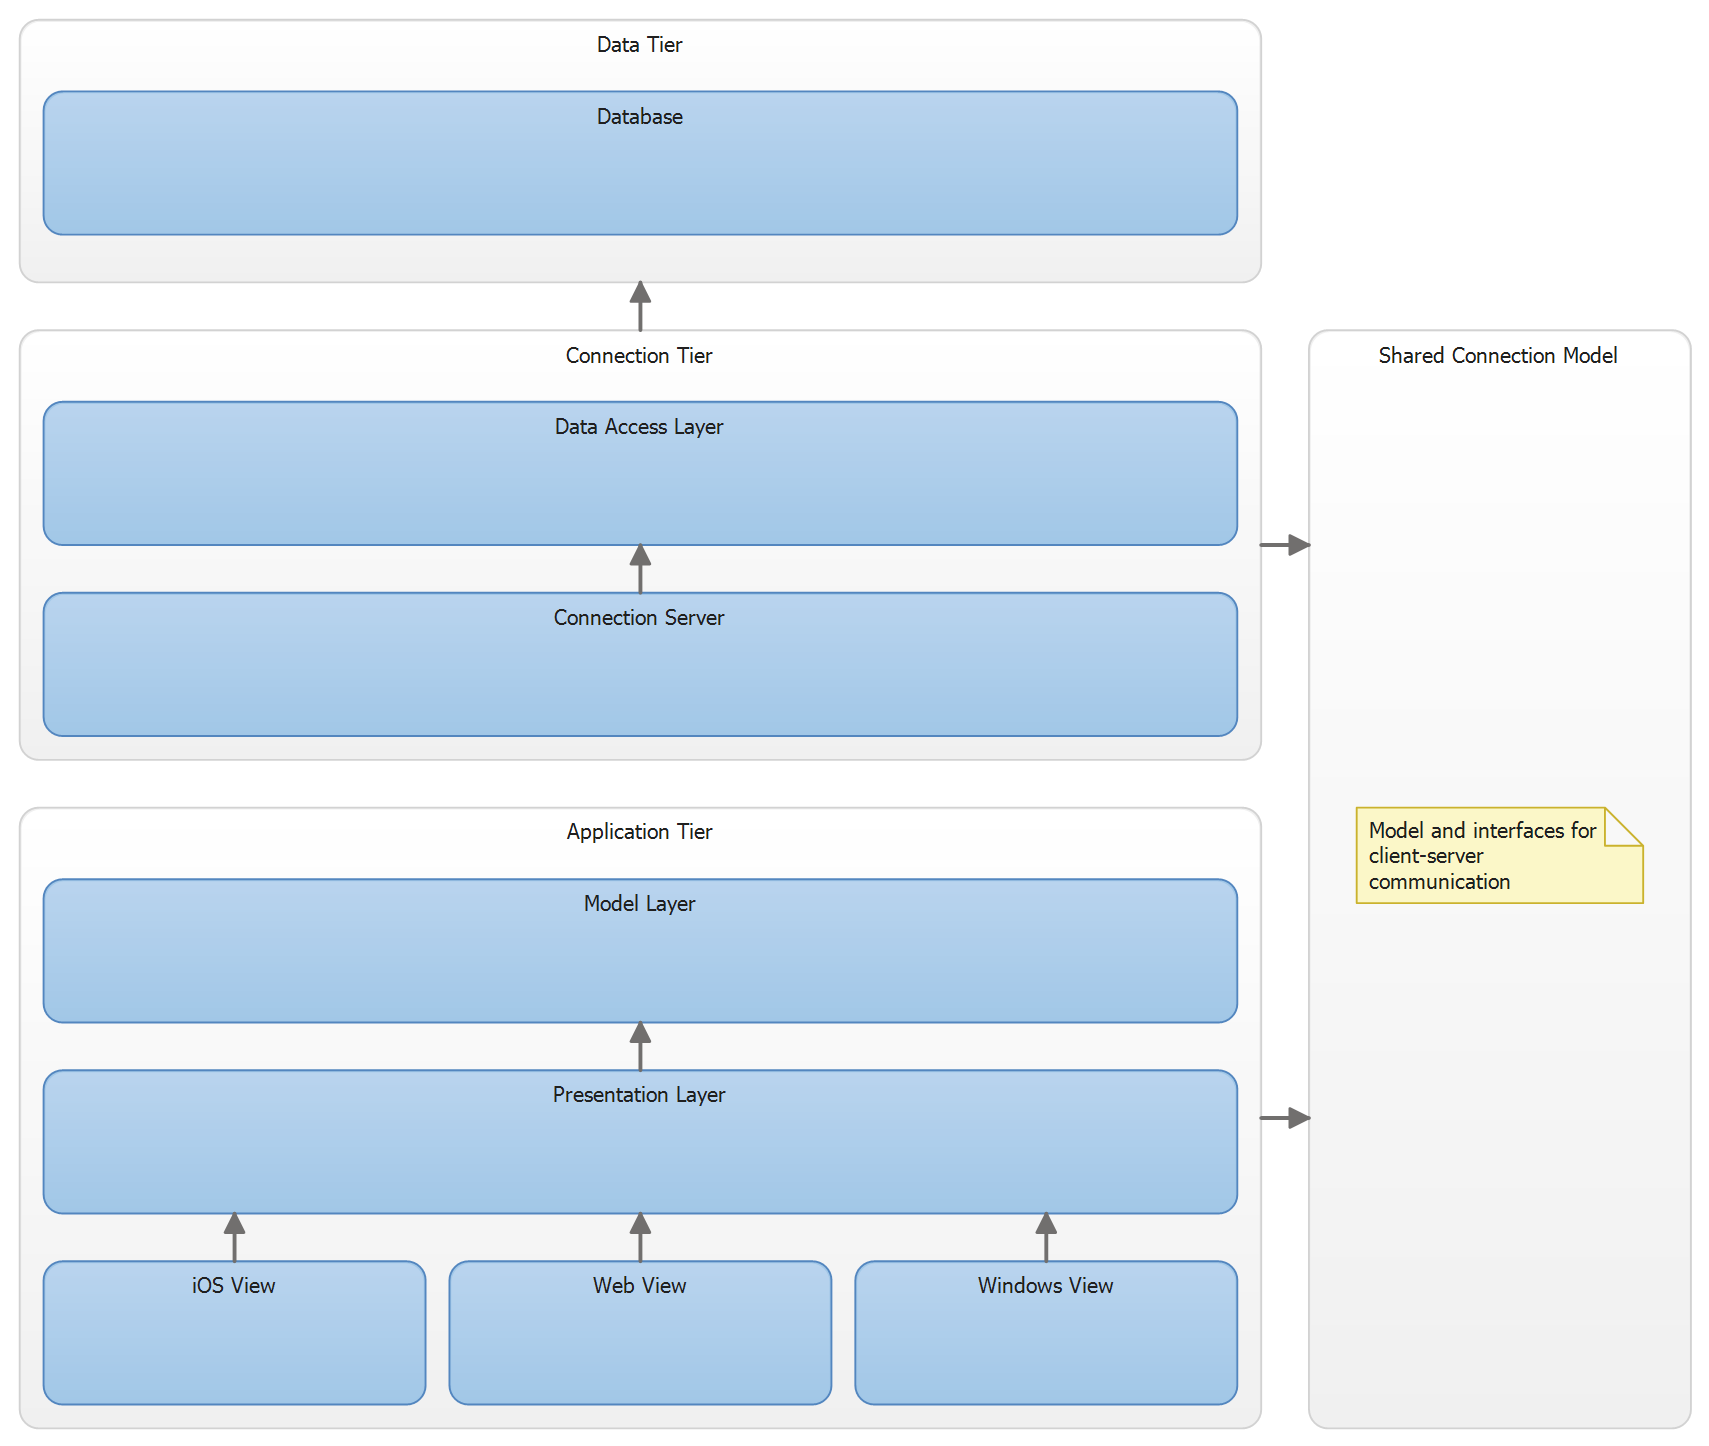
\includegraphics[width=0.9\linewidth]{figs/arkitektur/Smartpool_tiersnlayers}
	\caption{Tiers and layers}
	\label{fig:tiersnlayers}
\end{figure}

\subsection{Presentation Tier}
Det ønskes at afkoble view fra præsentationslogikken og modellen. Til det formål benyttes GUI arkitekturen MVP. Det bruges så viewet er afkoblet og dermed kan udskiftes. Det er gjort med henblik på, at genbruge præsentationslogikken på flere platforme. Arkitekturen understøtter dermed kravene til projektet om som minimum et Windows GUI, med mulighed for udvidelse til iOS og web. Application tier kommunikerer med Connection tier igennem en Shared Connection Model jf. figur \ref{fig:tiersnlayers}. 

\subsection{Business Logic Tier}

\subsection{Database Tier}

\section{4+1 Arkitektur Model}
Systemets arkitektur er beskrevet ved 4+1 modellen. \todo{fodnote eller ref til 4+1} 4+1 modellen består af en række views, som hver især henvender sig til forskelliger interessenter. I rapport bringes Logical view.

\subsection{Logical view}
Logical view beskriver funktionaliteten for systemets end-user. Logical view repræsenteres ved et Activity diagram. Figur \ref{ActivityDiagram} illustrerer et typisk brugsscenarie for en end-user. 
\begin{figure}
\centering
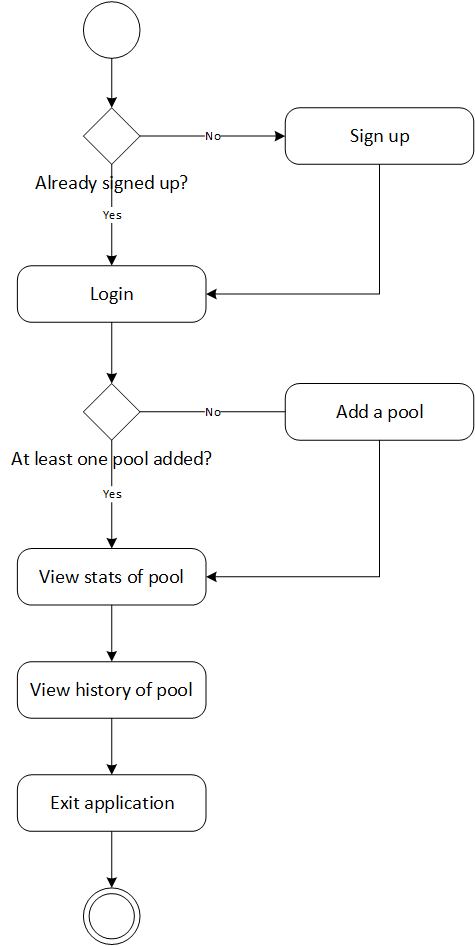
\includegraphics[width=0.55\linewidth]{figs/arkitektur/ActivityDiagram.PNG}
\caption{Activity diagram}
\label{fig:ActivityDiagram}
\end{figure}

De andre views for systemet forefindes i dokumentationen, de henvender sig primært til udviklere

